\documentclass[11pt]{article}

\usepackage{ijm}
\input{macros}

\title{$L_0$ regularization for subnational microsimulation calibration}

\author{
    María Juaristi\thanks{PolicyEngine. Corresponding author: maria@policyengine.org} \and
    Nikhil Woodruff\footnotemark[1] \and
    Ben Ogorek\footnotemark[1] \and
    Max Ghenis\footnotemark[1]
}
\date{}

\begin{document}

\maketitle

\begin{abstract}
Subnational microsimulation needs survey microdata that reproduce administrative totals across nested
geographies while staying usable inside a policy model. A fidelity-oriented pipeline can combine many
sources and add record-level variation, producing a candidate dataset rich enough to represent the
targets but too large to simulate. That dataset has to be reduced, and the question
is which records to keep.

We study this reduction as a sampling problem. Using $L_0$ regularization with the Hard Concrete
relaxation of \citet{louizos2018}, the method jointly selects which records to retain and assigns each a
positive weight, with selection driven by the calibration targets rather than drawn at random. The gates
make the retained-record count an explicit optimization variable, and soft and hard concentration controls
bound how large individual weights can grow. Because the optimization that selects records also calibrates
them, the reduced dataset continues to match its targets.

We implement the method within \populace{}, PolicyEngine's microsimulation data pipeline, and present a
proof of concept on its current full United States target surface. The run starts from 37{,}053 Ledger facts
and scores 31{,}534 materialized calibration targets, including 23{,}450 congressional-district targets, on
75{,}112 candidate households. Holding the candidate universe, target surface, and record budget fixed, we
vary only how records are chosen across target-informed $L_0$ selection and matched random-sampling
baselines, all scored by the same Populace capped weighted calibration loss. The experiment is therefore a
frontier between retained-record count and target fit, not a holdout exercise. On the current full target
surface, random sampling followed by gradient reweighting is the strongest baseline: informed $L_0$ plus an
ordinary post-selection refit improves substantially on the raw gated weights and nearly catches the
baselines at larger budgets, but it does not dominate the production loss. The useful finding is therefore
diagnostic rather than promotional. The machinery now runs the full surface, preserves the resulting weight
vectors, and exposes where target-informed selection needs work: better selected subsets, less weight
concentration, and robustness checks against classical calibration comparators.
\end{abstract}

\noindent\textbf{Keywords:} microsimulation, survey calibration, subsampling, $L_0$ regularization,
subnational analysis

\section{Introduction}
\label{sec:introduction}

Tax-benefit microsimulation models apply policy rules to household microdata to estimate fiscal and
distributional effects. At the national level, that usually means starting from a survey such as the
Current Population Survey (CPS), improving measured incomes and program participation, and adjusting
weights so the dataset reproduces known aggregates. Subnational work is harder. Analysts often want
estimates for states, congressional districts, or local areas, but the underlying survey was not
designed to support all of those geographies at once.

That gap matters in practice, because many reforms are proposed, administered, or debated below the
national level. A state tax proposal needs state-specific incomes, filing patterns, and benefit
participation. District-level analysis needs those same outcomes to aggregate correctly within each
district while staying consistent with state and national totals. A usable subnational dataset
therefore has to satisfy a hierarchical calibration problem rather than a single national one.

One way to meet that demand is to build a dataset that carries as much of the relevant variation as
possible. A pipeline can combine several surveys and administrative files, impute the variables that
any single source lacks, and place records across geographies so that local detail is present in the
candidate data. Each of these steps adds records, or variants of records. The result is a candidate
dataset rich enough to represent the variation the targets describe, and large enough that it
becomes expensive to store, calibrate, and simulate. A file with millions of active records supports
detailed subnational work but is slow to run; a much smaller file is easier to ship, but only if the
loss in fidelity is acceptable.

The candidate dataset therefore has to be reduced to a size that can be shipped and simulated, and
this paper treats that reduction as a sampling problem: given the large candidate universe and a
fixed record budget, which records should the final dataset keep, and what weight should each kept
record carry? The simplest answer is to draw a random subset
and reweight it to the targets. We study an alternative in which the selection itself is informed by
the targets.

The method is $L_0$ regularization with the Hard Concrete relaxation \citep{louizos2018}. Each
candidate record receives a gate that the optimizer can drive toward zero or one, and the expected
number of open gates enters the objective directly. Minimizing calibration error and the gate count
together selects a subset of records and fits their weights in one optimization. The retained-record
count becomes a quantity the optimizer controls rather than a fixed draw, and a separate weight
penalty limits how concentrated the fitted weights can become. In practical terms, one framework can
target a compact national dataset or a larger subnational dataset, at a chosen record budget, with
weights kept inside a usable range.

We situate this work in \populace{} \citep{populace2026}, PolicyEngine's pipeline for microsimulation
dataset construction. \populace{} passes a single weighted data structure through a sequence of
modular stages---source loading, imputation, geographic assignment, target construction, and
calibration---each implemented as a separate package operating on that shared structure. Because the
stages are modular, the data sources, the imputation model, the geographic assignment, and the
calibration method are interchangeable components rather than fixed code, and the calibration step
studied here is one such component. The paper describes the pipeline at the level needed to follow the
calibration step, and then describes the configuration used here.

This paper is a proof of concept on \populace{}'s current target surface: it asks whether
$L_0$ selection with Hard Concrete gates can produce a sparse, calibrated dataset on the targets
\populace{} assembles today. Local-area and subnational calibration are the production motivation for
the method and a future application of it, rather than results this paper presents.

The empirical question is whether informed selection earns its added complexity. We ask three
things. First, does $L_0$ selection reproduce the targets more accurately than random sampling,
survey-weight sampling, and combinatorial optimisation at the same record budget? Second, does the retained sample generalize, in the sense that it also
matches targets held out of the fit? Third, does the framework give usable control over the size of
the output, the geographic level it focuses on, and the magnitude of the fitted weights?

The rest of the paper follows that structure. Section~\ref{sec:background} places the work in the
literature on spatial microsimulation, survey calibration, and sparse selection.
Section~\ref{sec:data} describes the base microdata, the \populace{} pipeline, and the
administrative targets. Section~\ref{sec:methodology} presents the calibration method and the
sampling experiment design. Section~\ref{sec:results} reports the comparison against the sampling
baselines and the behaviour of the size, geography, and weight controls. Section~\ref{sec:discussion}
interprets those results and discusses their limits, and Section~\ref{sec:conclusion} concludes.

\section{Background and related work}
\label{sec:background}

\subsection{Subnational microsimulation and spatial reweighting}

Subnational microsimulation starts from a recurring problem: a national survey carries the
behavioural and demographic detail needed for policy modelling, but it does not contain enough
observations in every local area to support direct estimation. Spatial microsimulation addresses
that gap either by reweighting existing survey records or by building synthetic small-area
populations from aggregate constraints \citep{tanton2014review, odonoghue2014review}.

This distinction matters for the present work, because our pipeline is a reweighting system built on
observed CPS households. It places households across geographies to create local variants, but the
core problem remains the calibration of survey-based microdata to administrative targets, which keeps
calibration methods as the closest reference point.

The spatial microsimulation literature supplies further context. \citet{williamson1998},
\citet{huang2001}, and \citet{harland2012} describe combinatorial and synthetic-population
approaches that search over record assignments area by area. \citet{tanton2011} and
\citet{lovelace2016} discuss reweighting for small-area estimation and policy analysis. These
methods usually target one geographic layer at a time, whereas our setting asks one weighted dataset
to reproduce state and national targets together.

\subsection{Survey calibration}

Let $i = 1, \ldots, n$ index sampled units, let $d_i$ denote the initial design weight for unit $i$,
and let $\mathbf{x}_i \in \mathbb{R}^p$ denote the auxiliary variables used for calibration. Survey
calibration seeks adjusted weights $w_i$ whose weighted totals match known population totals:
\begin{equation}
    \sum_{i=1}^{n} w_i \mathbf{x}_i = \mathbf{T},
    \label{eq:calibration_constraint}
\end{equation}
where $\mathbf{T} \in \mathbb{R}^p$ is the vector of published totals \citep{deville1992,
sarndal2007}. The auxiliary variables may be counts, indicators, or continuous quantities such as
income components.

The subnational problem extends this setup in two ways. The target vector draws on several
administrative sources, so it mixes count and dollar constraints. The constraints are also nested by
geography: district totals should sum to state totals, which should sum to national totals after
uprating and reconciliation. At production scale this yields a large target system with substantial
collinearity across rows.

\subsection{Calibration estimators}

Two classical methods are the standard references for this kind of problem. Generalized regression
(GREG) minimizes a distance from the initial weights subject to the calibration equations
\citep{deville1992, sarndal2007}. It accepts quantitative targets directly and is well understood,
but it can return negative weights and becomes harder to solve as the target system grows and its
rows become collinear. Negative weights are acceptable in some estimation settings and awkward in a
microdata file meant for tax-benefit simulation, where a household is expected to represent positive
population mass.

Iterative proportional fitting \citep[IPF, or raking;][]{deming1940, ireland1968} adjusts weights
multiplicatively so that selected margins match published totals. It preserves non-negativity and
avoids matrix inversion, which makes it a natural choice for count-style margins. In spatial
microsimulation and population synthesis, raking is commonly paired with a sampling step in one of two
orders: draw a sample first and rake that fixed sample, or rake the full file first and integerise the
fractional weights into a finite population. Iterative proportional updating and related extensions
handle household and person margins simultaneously \citep{pritchard2012}. These raking-based workflows
are natural comparators for pruning methods on categorical margin surfaces. They are not direct
full-surface baselines here: classical IPF is built for non-negative categorical margins, whereas the
production target surface mixes counts, dollar totals, overlapping families, near-zero targets, and
hierarchical constraints. Generalized raking or entropy calibration can extend the idea to broader
linear constraints, but then the method becomes a general calibration optimizer rather than the
classical IPF workflow.

A third approach treats calibration as an optimization problem to be solved numerically. The two
methods above are special cases of one problem: \citet{deville1992} define the calibrated weights as
those closest to the design weights, under a chosen distance, subject to reproducing the targets,
with GREG and raking the closed-form solutions for particular distances. When the target system is
large, collinear, mixes count and dollar constraints, and restricts weights to be positive, the
classical Newton and Lagrange solvers become hard to apply or fail to converge, which motivates
minimizing the calibration objective directly. \citet{espuny2018} do so with a global optimization
that enforces the range restrictions on the weights explicitly, and minimum-distance reweighting has
long been used this way in tax microsimulation \citep{creedy2003}. At the scale of an enhanced
microdata file the practical solver is stochastic gradient descent: the weights are parameterized to
stay positive, typically in log space; a loss measures the relative discrepancy between the weighted
estimates and the targets; and an optimizer such as Adam \citep{kingma2015} minimizes it, which
scales to thousands of mixed, hierarchical targets without inverting a matrix. \citet{woodruff2024}
calibrate PolicyEngine's enhanced CPS in exactly this way.

These estimators answer a calibration question rather than a sampling one: given a fixed set of
records, they find weights that match the targets. The method studied here selects records and fits
weights at the same time, extending the gradient-based calibration just described with explicit
record selection. Classical calibration still matters for the comparison set, because it can be
combined with selection: sampling followed by raking is the classical reduce-then-calibrate analogue
to random sampling followed by gradient reweighting, while raking followed by integerisation is the
classical calibrate-then-reduce analogue to sampling from dense calibrated weights.

\subsection{Reducing microdata by selecting records}
\label{sec:reduction_methods}

Reducing a large candidate dataset to a fixed budget is a sampling problem with a long statistical
history, and several established methods reduce a microdata file by selecting actual records to match
known totals. They differ mainly in where calibration enters: before selection, after selection, or
inside the selection step itself. We review the broad option space because it defines what a reasonable
analyst might try: random sampling followed by calibration, calibration followed by integerisation,
raking-based variants of both, balanced sampling, combinatorial optimisation, and sparse optimization
relaxations. Not all of these are equally applicable to the production problem. The target surface here
is large, mixed, and hierarchical, so methods built for categorical margins or discrete area-by-area
searches are reference points rather than direct full-surface baselines. The matched-budget comparison
in Section~\ref{sec:methodology} therefore focuses on the tractable full-surface set: informed $L_0$,
informed $L_0$ followed by ordinary refitting on the selected records, random sampling with reweighting,
and survey-weight sampling. Raking-based reductions, convex sparse calibration, balanced sampling, and
combinatorial optimisation remain published comparators that motivate robustness checks where their
assumptions fit cleanly. We also note the coreset view from
machine learning, where a weighted subset is chosen so that a model fit on the subset approximates the
fit on the full data \citep{feldman2020coresets, bachem2017coresets}.

\subsubsection{Random sampling}

The simplest reduction draws records at random. Under simple random sampling without replacement each
record has inclusion probability $n/N$ and design weight $N/n$, and the Horvitz--Thompson estimator
recovers population totals without bias \citep{horvitz1952, cochran1977, sarndal1992}. A random
subsample preserves the conditional distribution of the data in expectation, but it does not
reproduce administrative totals, so it has to be calibrated after the draw. Random selection is also
the reference that the data-reduction literature treats as the genuine test: informativeness-based
schemes are measured against it \citep{ma2015leveraging}, and pruning methods in deep learning often
fail to beat it at high reduction ratios \citep{guo2022deepcore}. In our setting it is the
reduce-first, calibrate-after baseline, a random draw followed by gradient-descent reweighting to the
targets. Replacing the gradient reweighting step with raking gives the classical sampling-then-raking
workflow; it is directly comparable on a raking-compatible categorical margin subset, but not on the
full mixed count-and-dollar target surface without changing the problem into generalized calibration.

\subsubsection{Raking, survey-weight sampling, and integerisation}

A second approach calibrates first and reduces second. Given fractional weights from a calibration
step, survey-weight sampling selects records with probability proportional to those weights, which
turns a reweighted file into a finite, integer-weighted population that approximately preserves both
the calibrated totals and the distribution. This is unequal-probability,
probability-proportional-to-size sampling in the survey tradition \citep{hansen1943, horvitz1952},
applied to microsimulation as integerisation. The upstream calibration can be IPF/raking, GREG, or a
numerical optimizer; the downstream question is how to convert fractional weights into a finite file.
\citet{lovelace2013trs} catalogue the common integerisation methods and show that
truncate-replicate-sample reproduces the targets most accurately while fixing the reduced population
to an exact size; earlier top-up schemes are due to \citet{ballas2005}. Because the selection
probabilities are the calibration weights, survey-weight sampling presupposes a calibration step, so
in our comparison it is the calibrate-then-reduce baseline, with gradient descent supplying the
weights. A raking-then-TRS variant is the corresponding classical baseline on a categorical margin
surface, but it does not naturally extend to the full mixed production target surface without replacing
IPF with a broader calibration solver.

\subsubsection{Balanced sampling}

Balanced sampling selects a fixed-size sample whose Horvitz--Thompson estimates reproduce auxiliary
totals exactly or nearly exactly. The cube method of \citet{deville2004cube} is the standard
construction: it chooses inclusion indicators while preserving prescribed balancing equations, then
uses the resulting sample weights for estimation. This makes balanced sampling a target-aware
selection method rather than a post-sampling calibration method, and therefore a relevant published
neighbour of $L_0$ selection. Its fit to the present problem is not exact. Classical balanced sampling
usually treats the auxiliary totals as design constraints with predetermined inclusion probabilities,
whereas the production calibration surface here mixes categorical counts, dollar totals, and
hierarchical relationships and then fits positive weights after selection. Still, it is an important
reference point for the idea that the sample itself, not only its weights, can be chosen to preserve
known totals.

\subsubsection{Convex sparse calibration}

A final family keeps the continuous optimization setup but replaces the direct retained-record count
with a convex sparsity surrogate. An $L_1$ penalty on fitted weights, implemented with proximal
soft-thresholding, can drive weights exactly to zero while preserving the same calibration loss. This
is tractable on the full target surface and gives a useful ablation: it asks whether the value comes
from sparse joint selection in general or from the Hard Concrete $L_0$ relaxation specifically. Its
drawback is interpretive. The $L_1$ penalty shrinks weight magnitudes as well as encouraging zeros, so
its tuning parameter is not a direct retained-record-count control in the way the expected $L_0$ norm
is. We therefore treat it as a convex sparse analogue rather than as the primary sampling method.

\subsubsection{Informed selection}

These methods share the idea that a carefully chosen weighted subset can stand in for a larger
dataset, but they reach it differently: random sampling ignores the targets and repairs the gap
afterwards, survey-weight sampling inherits the targets from a prior calibration, balanced sampling
tries to preserve auxiliary totals through the sample design, and convex sparse calibration remains in
the same optimizer but changes the penalty. A fourth tradition makes selection itself the calibration:
combinatorial optimisation chooses a combination of records, with integer multiplicities, to match the
benchmark totals directly, searched with metaheuristics such as simulated annealing
\citep{kirkpatrick1983, williamson1998, voas2000}. It is the closest precedent for target-informed
selection, but it is discrete and gradient-free; we note it as related work rather than include it in
the matched-budget comparison. The method studied here also pursues the targets at selection, but with
a continuous, gradient-based relaxation that fits the selection and the weights jointly. The next
subsection sets out that relaxation.

\subsection{\texorpdfstring{$L_0$}{L0} regularization and the Hard Concrete distribution}

The $L_0$ norm counts the non-zero entries in a vector. Applied to record weights, it counts the
records that remain active, which is exactly the size of the retained sample. Selecting a subset of
a chosen size is therefore an $L_0$-penalized problem. The difficulty is that the $L_0$ norm is
non-differentiable and combinatorial, so it cannot be minimized by gradient descent in its raw form.

\citet{louizos2018} make the penalty differentiable by attaching a stochastic gate $z_i \in [0, 1]$
to each parameter and optimizing the expected $L_0$ norm. The gate is drawn from a Hard Concrete
distribution: a binary concrete (continuous-relaxation) variable stretched beyond the unit interval
and then clipped back into it. With a learned location parameter $\log \alpha_i$ and a fixed
temperature $\beta$, draw $u \sim \mathrm{Uniform}(0, 1)$ and set
\begin{align}
    s_i      &= \sigma\!\left(\frac{\log u - \log(1 - u) + \log \alpha_i}{\beta}\right), \\
    \bar{s}_i &= s_i (\zeta - \gamma) + \gamma, \\
    z_i      &= \min\!\big(1, \max(0, \bar{s}_i)\big),
    \label{eq:hardconcrete}
\end{align}
where $\sigma$ is the logistic function and $\gamma < 0 < 1 < \zeta$ are fixed stretch bounds.
Stretching $s_i$ from $(0, 1)$ to $(\gamma, \zeta)$ and clipping to $[0, 1]$ places point masses at
exactly $0$ and exactly $1$, so a gate can switch a record fully off or fully on while staying
differentiable in between.

Because the gate has a closed-form probability of being non-zero, the expected $L_0$ norm is
differentiable. The probability that gate $i$ is active is
\begin{equation}
    \Pr(z_i \neq 0) = \sigma\!\left(\log \alpha_i - \beta \log \frac{-\gamma}{\zeta}\right),
    \label{eq:l0penalty}
\end{equation}
and the $L_0$ penalty is the sum of these probabilities over all records,
$\sum_i \Pr(z_i \neq 0)$, which is the expected number of retained records; minimizing it pushes
gates toward zero. At test time the noise is removed and the gate is evaluated deterministically,
\begin{equation}
    \hat{z}_i
    =
    \min\!\left(
        1,
        \max\!\left(
            0,\,
            \sigma(\log \alpha_i)(\zeta - \gamma) + \gamma
        \right)
    \right),
    \label{eq:deterministic_gate}
\end{equation}
which returns an exact zero for any record driven far enough off and an exact one for any record driven
far enough on, with intermediate values in between. The exact zeros make the weight vector exactly
sparse; a record left with an intermediate gate is retained with its fitted weight scaled by the gate.

The two pieces depend on each other, which is the point worth stressing for readers new to this
construction. The $L_0$ penalty states the objective, that fewer active records are preferred, but
on its own it is not optimizable by gradient methods. The Hard Concrete gate makes that objective
differentiable, but on its own, without the penalty, it carries no pressure toward sparsity and
leaves every gate open. Used together they turn record selection into a term the optimizer can
minimize alongside calibration error. This is what makes the retained-record count a control
variable rather than the result of a separate thresholding step.

\subsection{\texorpdfstring{Convex sparse selection ($L_1$)}{Convex sparse selection (L1)}}
\label{sec:l1_background}

The $L_0$ count is the natural sparsity objective but a hard one. The standard convex surrogate replaces
it with the $L_1$ norm of the weights, $\lVert \mathbf{w} \rVert_1 = \sum_i |w_i|$, which is the LASSO of
\citet{tibshirani1996}. Adding the penalty to the calibration loss gives the convex program
\begin{equation}
    \min_{\mathbf{w} \ge 0}\; \mathcal{L}_{\mathrm{cal}}(\mathbf{w}) + \lambda_{L_1} \sum_{i=1}^{n} w_i,
    \label{eq:l1}
\end{equation}
where $\lambda_{L_1}$ sets the strength of the penalty and the weights are non-negative here, so
$|w_i| = w_i$. The $L_1$ norm is the standard tool for sparse regression and feature selection: unlike the
smooth $L_2$ (ridge) penalty, which shrinks coefficients but rarely sets them to zero, its corner at the
origin drives small coefficients to exact zeros. The program is convex and is minimized by proximal
gradient descent, each gradient step followed by a soft-thresholding step
$w_i \leftarrow \max(w_i - \tau,\, 0)$ that subtracts a fixed amount $\tau \propto \lambda_{L_1}$ from every
weight and clips at zero \citep{beck2009fista}, so a record whose pull on the targets does not clear the
threshold is dropped while the rest are kept and shrunk. The trade-off is structural: the single penalty
$\lambda_{L_1}$ controls both how many records survive and how much their weights shrink, because the same
norm that zeroes small weights also pulls the surviving ones toward zero, so forcing a small sample forces
heavy shrinkage on the records that remain. This convex arm is a natural next ablation for $L_0$: it
pursues the same target-informed sparse selection by a more stable route, and contrasting the two would
isolate what the $L_0$ gates buy by separating selection from weighting.

\subsection{Microsimulation dataset engines}

Beyond the calibration step itself, \citet{woodruff2024} embed that gradient-based reweighting in a
national pipeline that first imputes tax variables from the IRS Public Use File onto CPS records, and
that regularizes the weights with dropout rather than an explicit selection mechanism. The present
work keeps the gradient-based calibration but replaces dropout with the $L_0$ and Hard Concrete gates
of the previous subsection, so that record selection becomes explicit and the fitted weights are
exactly sparse. It also runs within \populace{}, a pipeline that
expresses dataset construction as a sequence of modular stages over a shared data structure. The data
sources, the imputation model, the geographic assignment, and the calibration method are
interchangeable components rather than fixed steps, which lets the same pipeline support different
countries and different methodological choices.
Section~\ref{sec:data} describes the pipeline and the configuration used here.

\section{Data}
\label{sec:data}

The calibration problem is defined by two inputs: the household microdata that form the candidate
universe, and the administrative targets the calibrated dataset must reproduce. This section
describes how \populace{} assembles the candidate microdata and how this study selects its targets.
The pipeline is the harness that produces the calibration problem; it is not itself the object of
evaluation.

\subsection{Populace as a construction pipeline}

\populace{} builds a microsimulation dataset by passing a single weighted data structure---a sampling
frame holding the records, their weights, and provenance---through a sequence of stages. Each stage is
a separate package that reads and writes that shared frame: it loads the source surveys, combines them
into one record universe, imputes missing variables, assigns geography, constructs the calibration
targets, and calibrates. Because every stage operates on the same structure, the imputation model and
the calibration method are components that can be swapped without rewriting the pipeline, and the
method studied here is one calibration option among those the pipeline supports.

This modular structure makes the candidate universe a property of the configuration rather than an
accident of the code: the source-loading and imputation stages set what information each record
carries, and calibration sets which records survive and at what weight. \populace{} follows a
generate-then-prune design, assembling the candidate universe once and pruning it to a deployable
budget at the calibration stage.

\begin{figure}[H]
    \centering
    \makebox[\textwidth][c]{%
        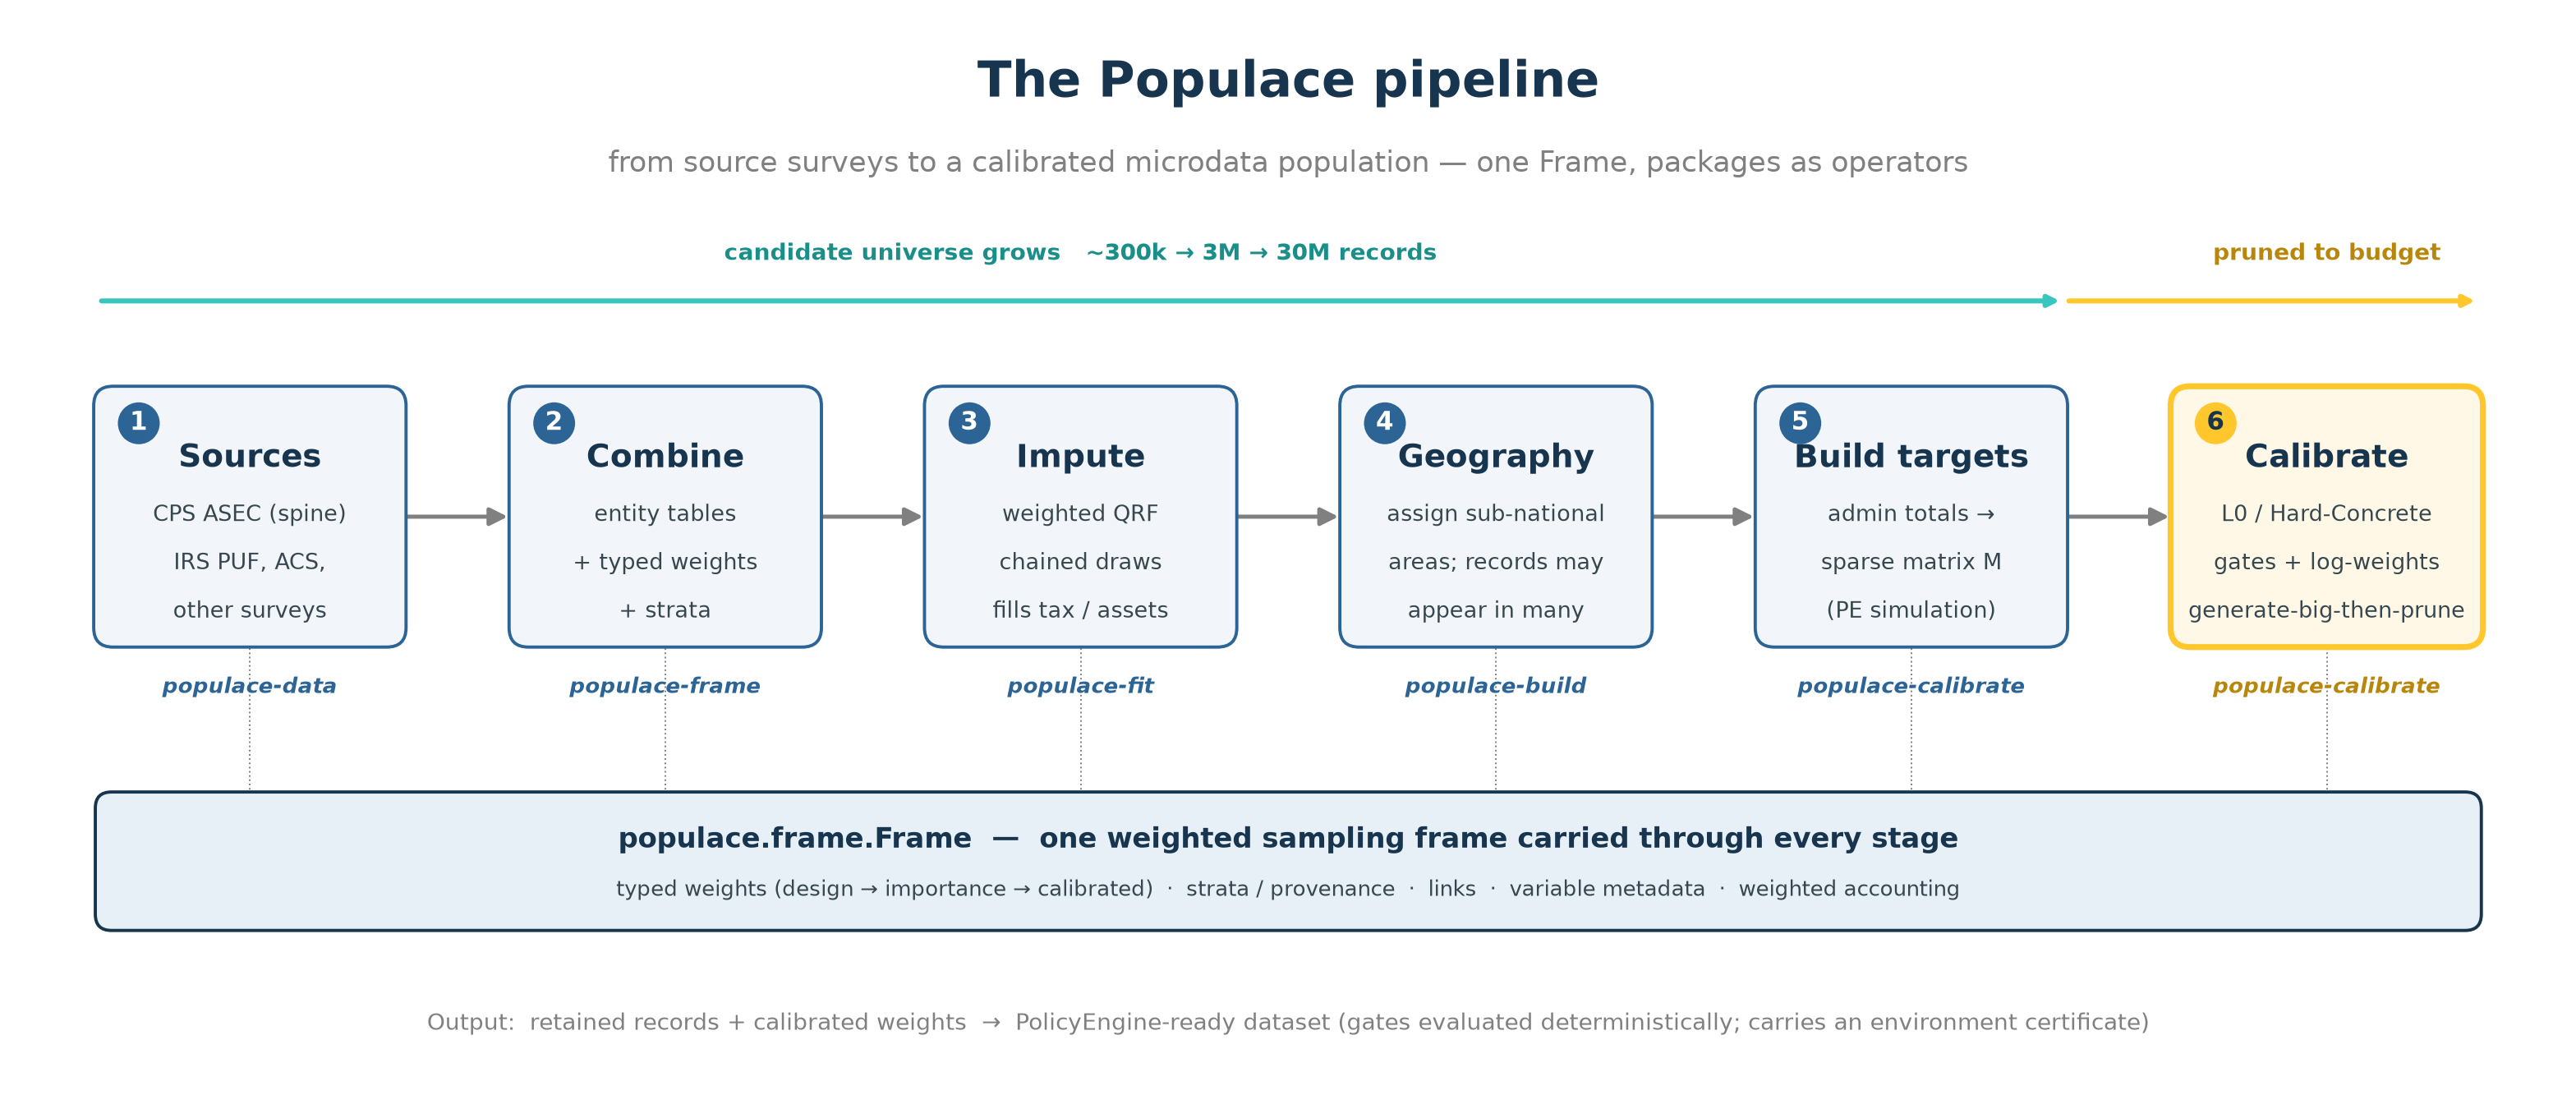
\includegraphics[width=1.18\textwidth]{figures/populace_pipeline}%
    }
    \caption{\populace{} pipeline for the configuration used in this paper: load and combine the
    source surveys, impute missing variables, assign geography, construct the calibration targets,
    and calibrate. The calibration stage is the focus of this paper.}
    \label{fig:pipeline}
\end{figure}

For this build the candidate universe is a three-year pooled ASEC support file for period 2024
(constructed as described below): 337{,}704 household records, one row per candidate household placement.
We pin the exact build for
reproducibility: \populace{} commit \texttt{558e46c1}, base H5 SHA-256 beginning
\texttt{ec290055}, Ledger facts SHA-256 beginning \texttt{82cd9e87}, and target-registry version
\texttt{5a22295b02b6}. The run resets household weights to a uniform prior before calibration, so the
comparison is about support selection and reweighting rather than inherited survey weights.

\subsection{Base microdata}

\subsubsection{Current Population Survey}

The primary source is the Current Population Survey Annual Social and Economic Supplement
\citep[CPS ASEC;][]{census2024}, a nationally representative household survey from the US Census
Bureau and the Bureau of Labor Statistics. The CPS provides demographic structure, household
relationships, labour income, transfer income, and reported participation in programmes such as
SNAP, Medicaid, SSI, and TANF.

The candidate universe is not a single survey year. To widen the support before pruning, \populace{}
pools the three most recently published CPS ASEC files---one per survey year---and ages the two earlier
vintages forward to the latest year, so all three are expressed at a common period, 2024 for this build.
Pooling three years rather than one substantially increases the number of candidate records and widens the
variation the frame carries, while aging keeps the older vintages comparable to the most recent one; the result is a
larger, richer candidate frame that still inherits the CPS survey design. This is the generate side of the
generate-then-prune setting: the pooled file is deliberately larger than the deployable dataset, and
calibration decides which of its 337{,}704 records survive.

The CPS is not a complete tax-benefit dataset on its own. Some tax variables are missing, others are
measured with error, and top incomes are imperfectly captured relative to tax records
\citep{burkhauser2012}. Benefit receipt is also underreported relative to administrative sources
\citep{meyer2015}. The pipeline therefore augments the CPS before calibration.

\subsubsection{Imputation from administrative and survey sources}

The pipeline enriches the CPS base by imputing variables from administrative and survey donors. It
imputes tax-return detail from the IRS Public Use File \citep[PUF;][]{bryant2023a} onto CPS records
following \citet{woodruff2024}: the PUF carries detailed tax-return information but lacks household
structure and demographic coverage, so quantile regression forests \citep{meinshausen2006quantile}
predict the PUF variables on the CPS; \citet{meyer2021} assess the accuracy of such
survey--administrative tax imputations. The imputation is sequential and regime-gated, drawing from a
weighted bootstrap, so later variables condition on earlier imputed values. The same machinery draws
further variables from the donors in Table~\ref{tab:donors} where the CPS is thin. Each step adds
variables to the existing households rather than new records, so the candidate universe stays at one
row per household.

\begin{table}[H]
\centering
{\tablefont
\begin{tabular}{@{}p{0.30\textwidth}p{0.60\textwidth}@{}}
\toprule
Donor source & Variables contributed (this build) \\
\midrule
CPS ASEC & Household and person structure, demographics, labour and transfer income, programme participation, unit assignment \\
IRS PUF (2015, uprated) & Itemized-deduction detail, QBI/SSTB components, partnership and S-corp income, selected tax detail \\
CPS ORG & Hourly wage, paid-hourly and union status, weekly hours, overtime inputs \\
SCF & Wealth and net-worth components \\
SIPP & Tips \\
MEPS-IC & Employer-sponsored insurance premiums \\
ACS (2022) & Rent (pre-subsidy) \\
CMS marketplace PUFs and CPS ASEC & ACA take-up and the benchmark-plan ratio \\
\bottomrule
\end{tabular}
}
\caption{Donor sources imputed onto the CPS base for this build, from the \populace{}-US release stage
manifest. The stages run in a fixed order, each conditioning on the variables already imputed.}
\label{tab:donors}
\end{table}

\subsubsection{Geography}

Each household carries a geographic identity. The CPS ASEC reports the household's state, and
\populace{} attaches congressional-district identifiers so the same frame can be calibrated against
national, state, and district targets. The current support file intentionally contains many more
candidate household placements than the final deployable file should retain. That is the build-big,
then-prune setting: \populace{} creates a support rich enough to cover the target surface, and the
calibration method decides which records survive.

\subsection{Calibration targets}

The target system combines aggregates from several administrative sources at the national, state, and
congressional-district levels. The headline experiment uses the full materialized target surface compiled
from the current \populace{} US fiscal registry: 37{,}053 Ledger facts produce 32{,}633 targets after
materialization against the candidate frame. Appendix~\ref{app:targets} lists the target families and
sources. The exact counts come from the run registry rather than from a pipeline-wide inventory.

\begin{table}[H]
\centering
{\tablefont
\begin{tabular}{@{}p{0.52\textwidth}l r@{}}
\toprule
Target family & Geographic level & Targets \\
\midrule
IRS Statistics of Income (\texttt{irs\_soi}) & National, state, district & 30{,}252 \\
Census population estimates (\texttt{census\_population}) & National, state & 936 \\
Medicaid and CHIP, CMS (\texttt{cms\_medicaid}) & National, state & 102 \\
ACA marketplace, CMS (\texttt{cms\_aca}) & State & 102 \\
SNAP, USDA (\texttt{usda\_snap}) & National, state & 52 \\
State income tax, Census STC (\texttt{state\_income\_tax}) & State & 44 \\
TANF, HHS ACF (\texttt{hhs\_acf\_tanf}) & National, state & 30 \\
Social Security OASDI, SSA (\texttt{ssa}) & National & 6 \\
JCT tax expenditures (\texttt{jct}) & National & 5 \\
CBO revenue projections (\texttt{cbo}) & National & 4 \\
Medicare, CMS (\texttt{cms\_medicare}) & National & 1 \\
\midrule
\textbf{Total} & & \textbf{31{,}534} \\
\bottomrule
\end{tabular}
}
\caption{Full materialized Populace target surface used in this study, by family and geographic level.
The surface contains 23{,}450 congressional-district targets, 7{,}615 state targets, and 469 national
targets.}
\label{tab:target_subset}
\tablenote{Counts are read from the full-surface run registry. In the headline experiment all targets,
including \texttt{cbo}, are fit and scored; holdout variants are supplemental diagnostics
(Section~\ref{sec:oos}). The source for each family is listed in Appendix~\ref{app:targets}.}
\end{table}


\section{Methodology}
\label{sec:methodology}

This section describes the calibration method that selects and weights records, and then the design
of the experiment that evaluates the method as a sampler.

\subsection{Selection and weighting as one optimization}

The calibration matrix $\mathbf{M} \in \mathbb{R}^{m \times n}$ maps $n$ candidate records to $m$
targets. Entry $M_{ji}$ is the contribution of candidate $i$ to target $j$: an indicator or count
for count targets, and a simulated tax or benefit value for dollar targets. The matrix is built from
\policyengine{} simulations evaluated under the policy rules that apply to each record's assigned
geography, and is stored in sparse form.

Given $\mathbf{M}$, the target vector $\mathbf{t}$, and a weight vector $\mathbf{w} \in \mathbb{R}^n$,
the optimizer minimizes
\begin{equation}
    \mathcal{L}(\mathbf{w}, \boldsymbol{\alpha}) =
    \frac{1}{m} \sum_{j=1}^{m}
    \min\!\left(\left|\frac{\hat{t}_j - t_j}{s_j}\right|, c\right) +
    \lambda_{L_0} \sum_{i=1}^{n} \bar{z}_i +
    \lambda_{L_2} \frac{1}{n} \sum_{i=1}^{n} \left(\frac{w_i}{w_{0,i}}\right)^2,
    \label{eq:loss}
\end{equation}
where
\begin{equation}
    \hat{t}_j = \sum_{i=1}^{n} M_{ji} w_i z_i.
    \label{eq:estimate}
\end{equation}
The first term is a calibration loss: the mean absolute relative error of the estimates against the
targets, where $s_j$ is the scale of target $j$ (its own magnitude $|t_j|$ for a pure relative error)
and $c$ caps the contribution of any single hard-to-fit target, so one badly conditioned target cannot
dominate the gradient. The implementation also admits optional per-target loss weights, which we leave
uniform here. The second term is the $L_0$ penalty: $\bar{z}_i$ is the expected activation of gate $i$
under the Hard Concrete relaxation \citep{louizos2018}, so $\sum_i \bar{z}_i$ is the expected number of
open gates --- the expected retained-record count --- and $\lambda_{L_0}$ sets how aggressively the
optimizer prunes. The third term is a soft concentration penalty: $\lambda_{L_2}$ multiplies the mean
squared ratio of each fitted weight to its initial weight $w_{0,i}$, which discourages the optimizer from
carrying the fit on a few heavily inflated records. It applies to the informed $L_0$ condition and is
left at zero for the baselines. The weights are parameterized in log space so the fitted weights stay
positive. This is the production optimizer that jointly fits positive log-weights and gates, rather than
a configuration that applies a gate on top of a separately fitted weight.

Read as a sampler, the three loss terms have distinct jobs, and a hard per-record constraint backstops
them. The calibration loss keeps the retained sample faithful to the targets, and because it is
relative, a one per cent error on a small target and on a large target count the same. The $L_0$
penalty sets the size of the retained sample. An $L_0$ penalty on its own, however, can reach a sparse
solution that is still unusable, because the optimizer can match the targets by placing very large
weights on a few retained records. The method governs that concentration through the ratio of each
fitted weight to its initial weight, $w_i / w_{0,i}$, with two complementary controls. The $L_2$ term
is a soft penalty on the mean square of that ratio: it discourages large inflations smoothly, and it is
the knob we sweep to trace the accuracy--concentration trade-off. \texttt{max\_weight\_ratio} is a hard
per-record cap on the same ratio: no fitted weight may exceed a fixed multiple of that record's initial
weight, enforced by clamping the log-weights after every optimizer step. It bounds the worst case rather
than the average. The two act at different points: the $L_2$ penalty shapes the whole weight distribution
during optimization, while the cap constrains the largest weight. Size and concentration are therefore
separate knobs: $\lambda_{L_0}$ sets how many records remain, and the $L_2$ penalty and
\texttt{max\_weight\_ratio} set how concentrated their weights may become. Together they let the pipeline
trade off calibration fit, sample size, and weight stability. The headline runs leave the
cap off and fix $\lambda_{L_2}$ at \tbc[the value chosen from the operability sweep of
Section~\ref{sec:results}]; tightening either bounds how much population any single record can carry, at
some cost to calibration fit. Appendix~\ref{app:hyperparameters} lists the full configuration, and
Algorithm~\ref{alg:l0} gives the optimization loop.

The gates and the weights are learned together: the gate decides whether a record is in the sample,
and the weight decides how much it counts. Because both are fit against the same calibration loss,
selection is informed by the targets: a record survives when keeping it helps match a target that
would otherwise be missed. This is the sense in which the method is a target-informed sampler rather
than a reweighting of a fixed random draw.

\subsection{From fitted weights to a dataset}

After optimization the gates are evaluated deterministically, so the retained-record count is read
from the solution rather than chosen by a post-hoc cutoff. The retained records and their weights are
assembled into a dataset for \policyengine{}. Appendix~\ref{app:assembly} summarizes the assembly
step, which matters operationally but is not the object of the experiment.

\subsection{Sampling experiment design}
\label{sec:experiment_design}

The experiment evaluates whether informed selection produces a better dataset than the alternative
samplers at the same record budget. From one candidate universe and one target set, we compare informed
$L_0$ selection against two matched-budget baselines, which span where calibration enters the reduction
(Section~\ref{sec:reduction_methods}):

\begin{itemize}
    \item \textbf{Informed $L_0$ sampling with Hard Concrete gates.} The method above selects records
    and fits weights jointly at a chosen budget, set through $\lambda_{L_0}$.
    \item \textbf{Random sampling with gradient-descent reweighting.} A random subset of the candidate
    universe of the same size is drawn, and its weights are fit to the same targets by gradient
    descent, using the same calibration loss without the gate term. This is the reduce-first,
    calibrate-after baseline.
    \item \textbf{Survey-weight sampling (Hansen--Hurwitz).} The full universe is first reweighted to the
    targets by gradient descent, and records are then drawn with probability proportional to those weights,
    \emph{with replacement}; each of the $n$ draws receives an equal share $W/n$ of the total weight $W$,
    and repeated draws accumulate on the same record. This is the unbiased Hansen--Hurwitz integerisation
    \citep{hansen1943} of the dense weights (it preserves their expectation at every budget), and is
    the calibrate-then-reduce baseline.
\end{itemize}

Combinatorial optimisation, the discrete gradient-free sibling of informed $L_0$ selection reviewed in
Section~\ref{sec:reduction_methods}, is not implemented in this study; the comparison here is the
three-way benchmark above.

Holding the candidate universe and the target set fixed isolates the effect of how records are
chosen. We sweep the retained-record budget across 2{,}000, 5{,}000, 10{,}000, 20{,}000, and 40{,}000 records,
from aggressive compression of the candidate universe up to a large fraction of it, and run each budget
over five calibration seeds (seeds $0$--$4$). Informed $L_0$ sets the achieved budget
at each grid point through its $\lambda_{L_0}$ bisection, and the baselines are matched to the same
retained count.

\subsection{Out-of-sample target evaluation}
\label{sec:oos}

A sampler can match the targets it is fit to and still generalize poorly. To test generalization, the
design separates the targets used to fit the weights from the targets used to score the result, and
holds out \emph{whole target families} rather than a random subset of targets. The reason is structural:
targets within a family nest (a national total is the sum of its state cells), so a random target split
leaks: a held-out cell is nearly determined by its retained siblings, which would overstate
generalization. Holding out a whole family removes that leakage.

The fixed holdout comprises the \texttt{cms\_medicaid}, \texttt{usda\_snap}, and \texttt{state\_income\_tax}
families, about \tbc[out-of-sample target count, $\approx$200] targets spanning three domains (Medicaid
enrollment and spending, SNAP, and state income tax). These families are held out of every method's fit
and scored only out-of-sample. Each held-out family keeps a \emph{sibling} family in the fit (ACA and
Medicare enrollment alongside Medicaid; the federal IRS SOI aggregates alongside state income tax), so
the test asks each method to reproduce a held-out family while a related family remains in the fit,
rather than orphaning a domain entirely. The \texttt{cbo} family is additionally held out as a \populace{}
validation-only family (forecast and aging projections used as diagnostics rather than contemporaneous
targets), so it is never fit. Of the \tbc[total target count] targets in the system,
\tbc[fit target count] are used to fit the weights.

As a stricter robustness check we also rotate whole families through the holdout in a family-grouped
five-fold design: the families are dealt into five folds balanced by target count, and each fold is held
out in turn. Because the folds hold out structurally different families rather than independent draws, we
report them per fold rather than as a single inferential test (Section~\ref{sec:results-generalization});
the rotation surfaces in particular the fold that holds out the dominant \texttt{irs\_soi} family.

\subsection{Evaluation metrics}
\label{sec:metrics}

Each run reports, for the scored targets in-sample and out-of-sample:
\begin{itemize}
    \item the \emph{median} absolute relative error as the headline accuracy measure, with the mean and
    maximum reported alongside but flagged as tail-sensitive;
    \item both a \emph{micro}-average over all scored targets (which the largest family, IRS SOI,
    dominates) and a family \emph{macro}-average (the mean of the per-family errors, giving each family
    equal weight regardless of how many targets it contributes);
    \item the effective sample size $\mathrm{ESS} = \left(\sum_i w_i\right)^2 / \sum_i w_i^2$ and the
    implied design effect, reported as a primary result rather than a footnote, because a sampler can fit
    the targets while concentrating population mass on a few records;
    \item the retained-record count, the largest fitted weights, and runtime.
\end{itemize}
Errors are reported by geographic level and by target family as well as in aggregate, because a sampler
can match national totals while missing local ones, or match one source while missing another.

A small number of targets have denominators so small that a single record can swing their relative error
past 100 per cent. We identify these structurally rather than by an arbitrary cutoff: target $j$ is
denominator-degenerate when its value is smaller than its \emph{identifiability floor}
$\max_i |M_{ji}|\, w_{0,i}$, the largest contribution any single record makes at its initial weight. For
such a target the absolute relative error reflects integer placement noise rather than calibration
quality. Rather than winsorize or trim the error distribution, we \emph{name} these targets in a one-time
audit and report a targeted-removal sensitivity (the mean recomputed with exactly those named targets
dropped) beside the full mean, so the effect of the degenerate targets is visible and attributable.
Target counts are read from each run's manifest.

\section{Results}
\label{sec:results}

The results answer the production question directly: with the candidate universe, target surface, and
record budget fixed, which retained weight vector best fits the current \populace{} target surface? All
methods are scored on the full set of 32{,}633 materialized targets, using the penalty-free Populace
objective loss in Equation~\ref{eq:loss_cal}. The run reported here is a matched full-scale probe rather
than a full budget frontier: a normalized $L_0$ penalty selects a sparse support, the same retained count
is used for the post-$L_0$ refit and sparse baselines, and an epoch-matched dense no-$L_0$ calibration
anchors the comparison. Raw absolute-relative-error (ARE) summaries, effective sample size, and max weight
are reported as diagnostics around the headline loss.

\subsection{The full-surface matched probe}

Figure~\ref{fig:objective_frontier} is the headline result. On the current three-year ASEC support file,
the normalized $L_0$ penalty selects 57{,}240 of 337{,}704 candidate households, or 17.0\% of the
candidate universe. The raw gated $L_0$ weights are not the right publication weights: scored after
thresholding, they reach a Populace objective loss of 9.86\%. Removing the gates and refitting ordinary
calibration weights on exactly the selected records lowers that loss to 4.74\%. A dense no-$L_0$
calibration using all 337{,}704 records and the same 1{,}500-epoch optimizer budget reaches 5.07\%. A
random subset of the same size as the $L_0$ support, followed by the same 1{,}500-epoch gradient
reweighting, reaches 7.55\%. A random subset of the dense calibrated weights, scaled back to the dense
total but not refit, reaches 24.24\%.

The practical interpretation is that the $L_0$ selector is doing useful support-selection work, but the
post-selection refit is essential. The selected support gives a lower finite-budget optimizer loss than
the full dense run at 1{,}500 epochs and fits the full target surface much more closely than a random
support of the same size. This should not be read as a claim that the dense feasible set is worse: the
dense no-$L_0$ loss is still declining at the end of the 1{,}500-epoch budget. The defensible claim is that
this $L_0$ support gives a better sparse support and a faster route to low loss under the completed
optimizer budget. The current evidence should still be read as a single fixed-penalty probe, not as proof
that this exact penalty is optimal: the next sweep needs to trace the normalized penalty across multiple
retained counts and concentration settings.

\begin{figure}[H]
    \centering
    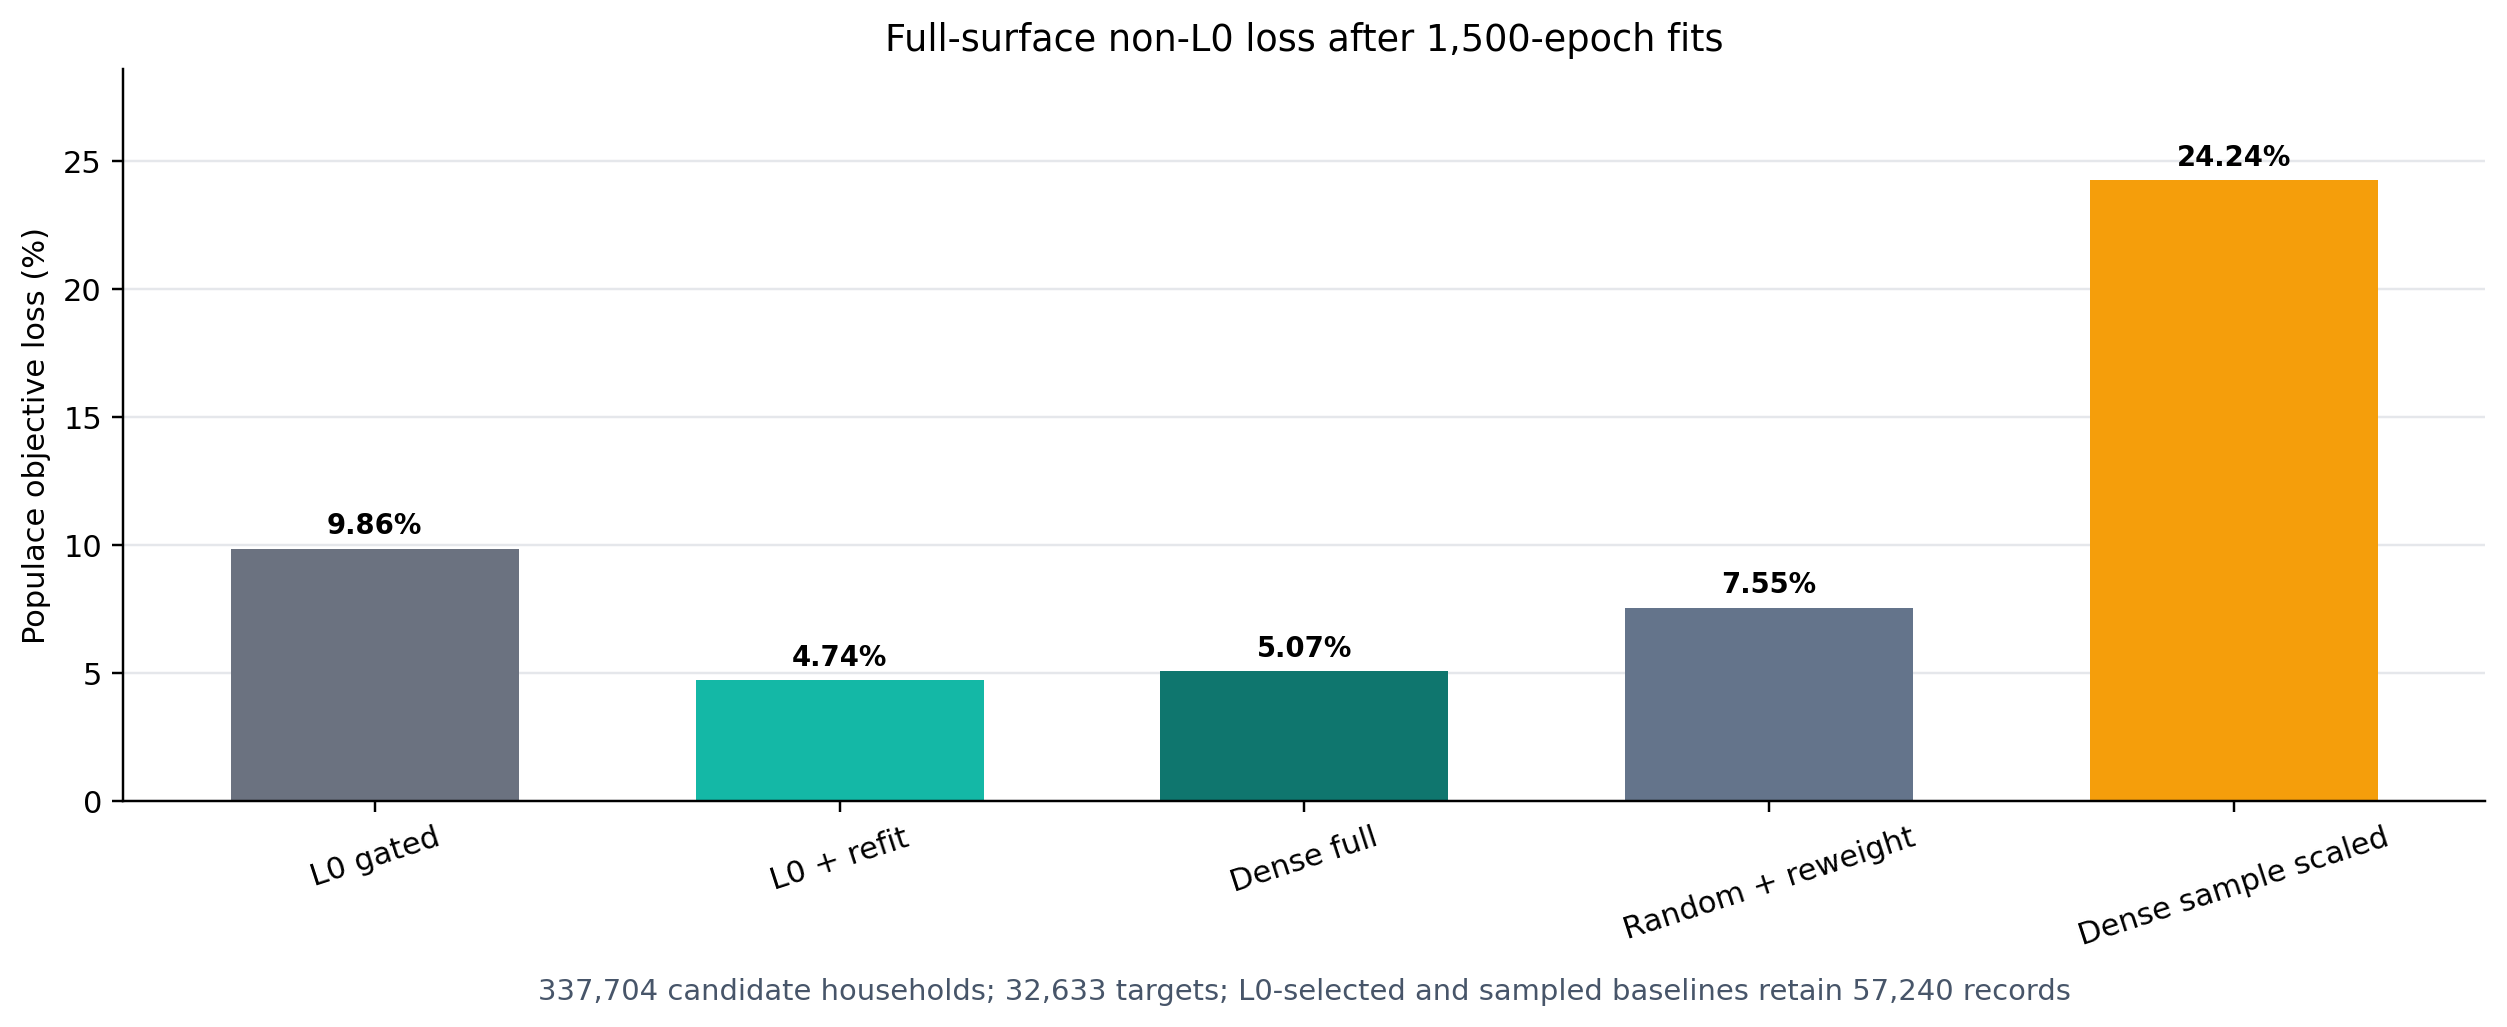
\includegraphics[width=0.96\textwidth]{figures/f0_objective_frontier}
    \caption{Full-surface Populace objective loss in the matched probe. The objective is the capped,
    target-weighted calibration loss in Equation~\ref{eq:loss_cal}, evaluated on each method's final
    retained/sampled weight vector and excluding sparsity or concentration penalties. The $L_0$ run uses a
    normalized penalty share of 0.8, equivalent to raw $\lambda_{L_0}=2.37\times10^{-6}$ for 337{,}704
    candidate households.}
    \label{fig:objective_frontier}
\end{figure}

Table~\ref{tab:sampling_comparison} reports the same comparison with raw ARE and weight diagnostics. The
median ARE gives a different view from the capped objective: dense no-$L_0$ has the lowest median ARE
(0.56\%), while the post-$L_0$ refit is close (0.89\%) and has the lowest capped Populace loss. Random +
reweight has 6.70\% median ARE, raw gated $L_0$ has 11.66\%, and the dense random scaled sample has
55.24\%. The mean ARE remains much larger because a small tail of difficult IRS targets can have very
large relative misses even when the capped Populace loss is low.

\begin{table}[ht]
\centering
{\tablefont
\resizebox{\textwidth}{!}{%
\begin{tabular}{p{0.20\textwidth}rrrrrr}
\toprule
Method & Budget & In-sample median ARE (\%) & Out-of-sample median ARE (\%) & Out-of-sample mean ARE (\%) & ESS & Max weight \\
\midrule
Informed $L_0$ & 10{,}000 & \multicolumn{5}{c}{\tbc[from \texttt{expanded-5seed}]} \\
Random + reweight & 10{,}000 & \multicolumn{5}{c}{\tbc[from \texttt{expanded-5seed}]} \\
Survey-weight (Hansen--Hurwitz) & 10{,}000 & \multicolumn{5}{c}{\tbc[from \texttt{expanded-5seed}]} \\
\bottomrule
\end{tabular}
}
}
\caption{Informed $L_0$ sampling against the two matched-budget baselines at a representative budget (the
$\sim$10{,}000-record anchor of Figure~\ref{fig:budget_frontier}). All methods share the candidate
universe, the target set, and the fixed family-level holdout, and differ only in how records are
selected. ARE is absolute relative error across the scored targets; the median is the headline read and
the mean is reported alongside as tail-sensitive. ESS is the Kish effective sample size, reported as an
output diagnostic because a sampler can fit the targets while concentrating population mass on a few
records. Cells are the cross-seed summary over five seeds.}
\label{tab:sampling_comparison}
\tablenote{The matched record budget and target counts are read from each run's manifest; the
out-of-sample columns score the held-out families. The survey-weight baseline is the unbiased
Hansen--Hurwitz integerisation (probability-proportional-to-size with replacement). Informed $L_0$ runtime
includes the eight-step budget bisection that sets $\lambda_{L_0}$; the baselines are run once at the
matched budget. Runtime and the family macro-average are reported in the run summary.}
\end{table}


Table~\ref{tab:paired_comparison} expresses the comparison on the headline loss scale. Relative to dense
no-$L_0$, the post-$L_0$ refit lowers the completed-run Populace objective by 6.4\%. Relative to random +
reweight, it lowers the objective by 37.2\%. Relative to the raw gated $L_0$ weights, it lowers the
objective by 51.9\%. The comparison isolates the value of the support and the refit: keeping dense weights
on a random retained set and merely scaling them back to total mass performs poorly, so a sparse file still
needs a reweighting step.

\begin{table}[H]
\centering
{\tablefont
\begin{tabular}{lrr}
\toprule
Comparison & Loss difference (pp) & Relative loss change \\
\midrule
Informed $L_0$ + refit vs. dense no-$L_0$ & $-0.33$ & $-6.4\%$ \\
Informed $L_0$ + refit vs. random + reweight & $-2.81$ & $-37.2\%$ \\
Informed $L_0$ + refit vs. raw informed $L_0$ & $-5.12$ & $-51.9\%$ \\
Dense random sample, scaled vs. dense no-$L_0$ & $+19.17$ & $+378.3\%$ \\
\bottomrule
\end{tabular}
}
\caption{Matched loss comparisons for the full-surface probe. Negative values favour the method named
first. Differences are in percentage points of the capped, target-weighted Populace objective loss.}
\label{tab:paired_comparison}
\tablenote{This table is descriptive because the current matched full-scale run uses one seed and one
normalized $L_0$ penalty. Dense no-$L_0$ and the post-selection/refit baselines all use 1{,}500 optimizer
epochs, but dense no-$L_0$ is still slowly declining at the end of that budget.}
\end{table}


\subsection{Size and concentration}
\label{sec:results-controls}

The normalized penalty gives a usable size control in this probe. We parameterize the sparsity price as a
share of the mean calibration loss, $\lambda_{\mathrm{share}}\sum_i\bar{z}_i/n$, rather than as an
unscaled raw coefficient. With $\lambda_{\mathrm{share}}=0.8$, the optimizer retained 57{,}240 records.
This scaling matters operationally: the same raw coefficient has very different meanings when the
candidate universe changes from tens of thousands to hundreds of thousands of records.

The selected support is more concentrated than the full dense calibration but better conditioned than the
matched random sparse baselines. Dense no-$L_0$ has an effective sample size of 5{,}970 and a maximum
weight of 579{,}298. The post-$L_0$ refit has ESS 4{,}726 and maximum weight 913{,}836. Random + reweight
has lower ESS, 2{,}480, and a higher maximum weight, 1{,}163{,}939; the dense random scaled sample is worse
again, with ESS 981 and maximum weight 2{,}176{,}121. The raw gated $L_0$ weights have higher ESS,
6{,}879, but worse target fit, which is why the refit is the publishable sparse variant.

\begin{figure}[H]
    \centering
    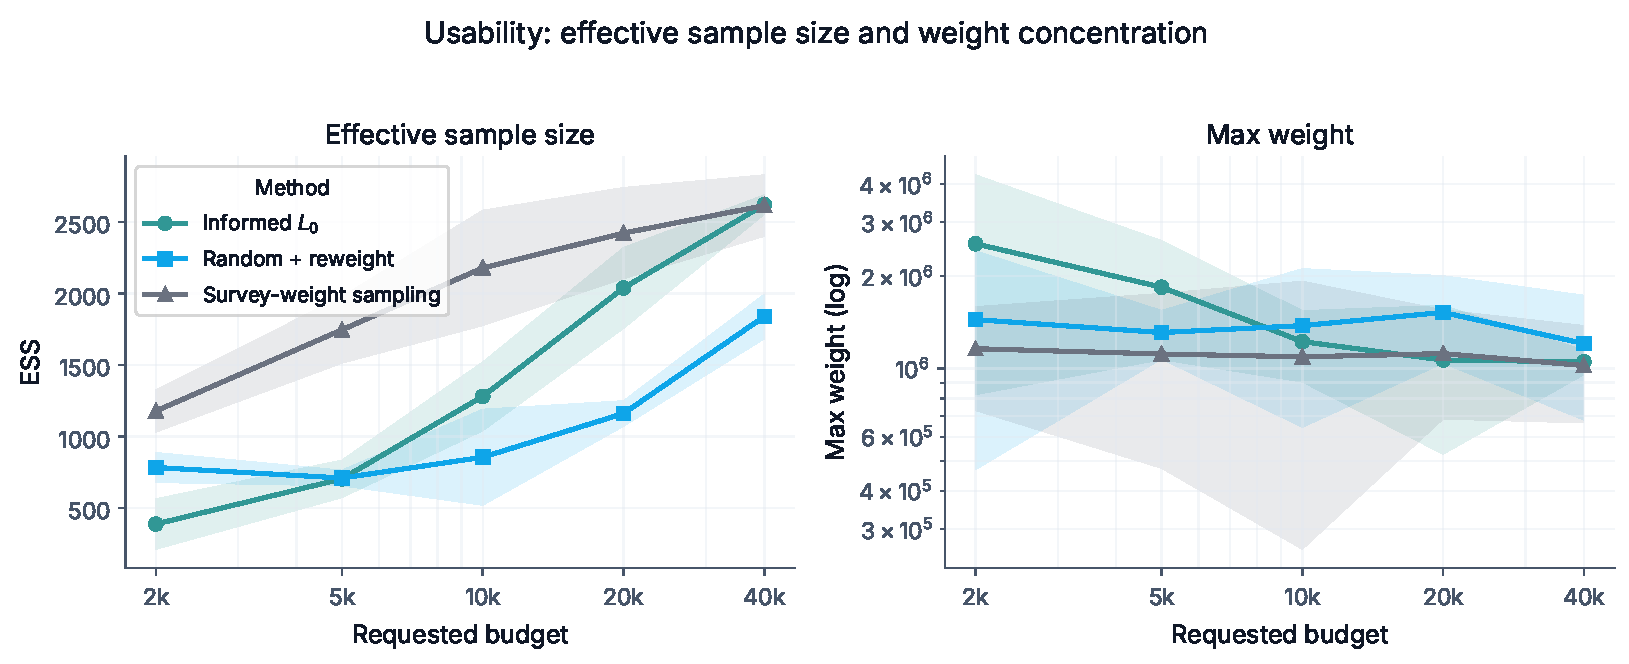
\includegraphics[width=\textwidth]{figures/f2_usability}
    \caption{Weight concentration in the matched full-surface probe. Effective sample size and maximum
    weight are computed on each method's final retained/sampled weight vector. Dense no-$L_0$ retains all
    337{,}704 records; the other sparse rows retain 57{,}240 records.}
    \label{fig:usability}
\end{figure}

\subsection{Accuracy by geography}

Table~\ref{tab:calibration_accuracy} breaks the post-$L_0$ refit diagnostics down by geography. The fit is
strongest at the state level, where median ARE is 0.31\%, followed by national targets at 1.30\% and
district targets at 1.48\%. District targets are the intended stress test for the method: they are the
largest part of the target surface, and they are the reason \populace{} needs to build a large candidate
universe before pruning it.

\begin{table}[H]
\centering
{\tablefont
\begin{tabular}{lrrrr}
\toprule
Geographic level & Targets & Median ARE (\%) & Mean ARE (\%) & Max ARE (\%) \\
\midrule
National & 478 & 1.30 & 20.12 & 557.29 \\
State & 7{,}815 & 0.31 & 86.36 & 122{,}712.20 \\
Congressional district & 24{,}340 & 1.48 & 85.29 & 162{,}495.93 \\
\midrule
\textbf{All scored targets} & 32{,}633 & 0.89 & 84.64 & 162{,}495.93 \\
\bottomrule
\end{tabular}
}
\caption{Calibration accuracy by geographic level for the Informed $L_0$ + refit run at 57{,}240
records, measured as absolute relative error (ARE) across the full target surface. The median reports the
typical target's error; the mean and maximum are tail-sensitive diagnostics.}
\label{tab:calibration_accuracy}
\tablenote{Raw ARE is undefined for 26 IRS SOI national targets where both target and achieved values are
zero; those rows are included in the target count and the Populace loss but omitted from the raw ARE
summary.}
\end{table}


\subsection{Raw-error tails}
\label{sec:results-degenerate}

The Populace objective is the headline score because it is capped and target weighted; raw ARE summaries
are supplemental. In the matched probe, raw ARE is defined for 32{,}607 of the 32{,}633 scored targets.
The remaining 26 rows are IRS SOI national targets with both target and achieved values equal to zero, so
they are omitted from raw relative-error summaries but do not affect the capped loss. Among the defined
rows, the post-$L_0$ refit has a 0.89\% median ARE and an 84.6\% mean ARE. The gap between the median and
the mean is the reason the paper leads with the Populace loss and reports raw ARE only as a diagnostic.

\subsection{Cost}

The matched probe took 39.4 minutes for the $L_0$ selection run. The post-selection refit then added about
9.5 minutes, for a combined 48.9 minutes reported in the artifact. Dense no-$L_0$ took 38.7 minutes for
1{,}500 epochs, random + reweight took 7.3 minutes, and the dense random scaled sample required no extra
optimization beyond the dense fit. The selector is therefore computationally expensive, and the dense run
is still slowly declining at the endpoint. The accuracy gain over dense and random + reweight is large
enough in this probe to justify a broader normalized-penalty sweep, but not enough to skip the next
robustness work: more penalties, longer dense convergence checks, more candidate-support regimes, and
concentration controls.

\section{Discussion}
\label{sec:discussion}

\subsection{What the sampling comparison establishes}

The comparison against the matched-budget baselines turns on the record budget, and on which error
statistic is read. Under aggressive compression, where the budget is too small for a random draw to span
the target system, informed $L_0$ selection holds the lowest error because the gates spend the budget on
the records the targets constrain. As the budget grows the methods converge: on the headline median the
edge passes to random + reweight once almost any subset can be reweighted to fit (near 5{,}000 records
here), while on the tail-sensitive mean informed $L_0$ stays ahead at every budget, because it removes the
seed-to-seed instability that swings a small random or survey draw's mean by thousands of per cent
(Section~\ref{sec:results}). The result is graceful degradation under compression rather than a blanket
accuracy win, and the budget at which the median crossover happens is itself a finding. Past it the case
for informed $L_0$ rests on its controls, on its near-zero generalization gap, and on the tail it keeps
bounded, rather than on a median accuracy gap. It removes the risk of a poor random draw and sets the
dataset size, the geographic emphasis, and the weight concentration through explicit parameters in one
optimization. That control matters most in the build-big-then-prune setting the method is designed for,
where a pipeline assembles a candidate universe far larger than it can ship and must reduce it to a fixed
budget under subnational calibration targets; this study tests the national and state surface, and the
subnational case is left to future work. Reporting out-of-sample error on held-out families keeps the
comparison honest, since any method matches the targets it was fit to more tightly than ones it never saw.

The convex $L_1$ arm sharpens the contrast. $L_1$ pursues the same target-informed sparse selection, but
through a single penalty that must both decide which records to drop and how much to shrink the survivors. Forcing roughly two thousand of seventy-five thousand records to survive demands a
large penalty, which soft-thresholds the retained weights toward zero and collapses the calibration fit:
its out-of-sample median ARE is pinned near 100\% at the tightest budgets and its mean runs to several tens
of thousands of per cent, recovering toward informed $L_0$ only once the budget is loose enough that little
shrinkage is needed (Figure~\ref{fig:budget_frontier}). Informed $L_0$ avoids this because the Hard
Concrete gate and the fitted weight are separate variables: the gate decides membership and the weight is
free to take whatever positive value the targets require. Decoupling selection from shrinkage is what lets
$L_0$ degrade gracefully where the convex relaxation does not, and it is the core of the $L_0$-versus-$L_1$
comparison. $L_1$ is more stable to optimize and can be the better choice where sparsity is not forced
hard; the case for $L_0$ here rests on the joint selection-and-weighting framing and the explicit control
over the retained count, not on a claim that it is the most accurate sparse method in every setting.

\subsection{What the controls establish}

The second contribution is operational: the same framework produces datasets of different sizes by
changing the $L_0$ penalty, focuses on a geographic level by weighting its targets, and shapes the
weight distribution through two concentration controls, a soft $L_2$ penalty and a hard per-record cap.
We treat the last of these as a measured frontier rather than a fixed setting: sweeping the $L_2$ penalty
traces what tightening concentration (raising the effective sample size and lowering the largest weights)
costs in calibration accuracy, so an operator can choose a point on that trade-off rather than accept
whatever concentration the unconstrained fit produces. A random-sampling baseline
can also produce a dataset of a chosen size, but it cannot make the choice of records respond to the
targets, and it controls concentration only through the reweighting step. The value here is that size,
geographic focus, and weight stability are set through explicit parameters in one optimization rather
than through separate heuristics.

\subsection{Trade-offs and limitations}

The method does not remove modelling judgment, and several choices stay consequential; the optimizer's
hyperparameters are one such choice, reported in full in Appendix~\ref{app:hyperparameters}.

\subsubsection{Target selection}

The target set is a prioritized subset, not a complete inventory. The reasons for including each
family are stated in Appendix~\ref{app:targets}, and the empirical claims are tied to the exact
targets in each run's manifest. A different target set could change the comparison, and the paper
does not claim the chosen set is maximal.

\subsubsection{When informed selection helps}

Informed selection should help most when the targets are specific and local, so the choice of
records matters. When the targets are few and broad, a random draw may already contain the records
needed to match them, and the advantage of informed selection narrows. The paper reports the regimes
it tests and does not extrapolate beyond them.

\subsubsection{Weight concentration and effective sample size}

Matching a demanding fiscal target system from a uniform prior can require the optimizer to load a
large share of the population onto a small number of records, so the effective sample size can fall
well below the retained-record count even when the calibration fit is good. That concentration is
acceptable for the aggregates the dataset is calibrated to, but it is a real cost for any downstream
estimand that is sensitive to the weight distribution. We expose the cost rather than hide it: the
effective sample size and the largest weights are reported as primary results, and the $L_2$ sweep
shows how much accuracy raising the effective sample size costs. That cost depends on the budget. At
40{,}000 records $\lambda_{L_2}=10^{-4}$ raises the effective sample size by about seventy per cent (from
3{,}803 to 6{,}482) for under two points of median accuracy, while at the tightest budget it inflates the
error tail instead. The penalty is worth applying at large budgets and not at tight ones, which is why we
report the un-penalised frontier as the accuracy result and the penalty as a separate operability setting.

\subsubsection{Generalization across target families}

Holding out whole families is a deliberately hard test of generalization, harder than holding out a
random subset of targets, and it need not flatter any method. On the fixed holdout, informed $L_0$
generalizes with almost no gap between its in-sample and out-of-sample median error, while random +
reweight fits the in-sample targets far more tightly but pays about a thirty-point gap on families it
never saw; informed selection trades in-sample fit for a sample that carries over. The stricter family
rotation is less forgiving. On the target-weighted mean across folds the ranking favours the baselines,
but the gap is confined to the fold that holds out the dominant \texttt{irs\_soi} family: with 71\% of the
targets removed, every method's mean is dominated by a few near-zero-denominator targets, and the fold
medians stay close. We read the rotation as a limitation to be reported per fold rather than as a single
headline number, and widening the held-out surface further is left to future work.

\subsubsection{Degenerate targets and the choice of error metric}

A handful of targets have denominators small enough that one record's placement swings their relative
error past 100 per cent, which inflates the mean absolute relative error without reflecting calibration
quality. Rather than winsorize or trim the distribution by an arbitrary cutoff, we lead with the median,
name the affected targets in a one-time audit, and report the mean recomputed with exactly those named
targets removed. This keeps the metric honest and the dropped targets visible and attributable, but it
does mean the headline accuracy figure depends on a stated, auditable choice rather than on the raw mean
alone.

\subsubsection{Computational cost}

Building the calibration matrix and running gradient-based optimization cost more than a small
classical calibration, and informed $L_0$ adds the eight-step budget bisection on top of a single fit;
Appendix~\ref{app:cost} reports the runtime each method reaches against the accuracy it buys. That cost
is justified only when the problem requires it, which is why the comparison against a simpler
random-sampling baseline matters.

\subsection{Generalizability}

The data engineering here is specific to the United States, but the question is general. Many
microsimulation projects combine sources into a candidate dataset larger than they can ship, and then
have to reduce it. Where the reduction has to respect calibration targets and keep weights usable,
framing it as informed sampling, rather than as a random draw followed by reweighting, may carry over
to other countries and other engines. \populace{} makes that portability concrete, since the method
is a configuration choice rather than a fixed pipeline.

\section{Conclusion}
\label{sec:conclusion}

This paper studies $L_0$ regularization as a way to subsample a large microsimulation dataset down to
a usable size. The problem arises because a pipeline built for fidelity combines many sources and
adds record-level variation, which produces more candidate records than a deployable dataset can
hold. The reduction to a fixed budget is a sampling choice, and the paper treats it as one.

The method uses Hard Concrete gates to select records and fit their weights in one optimization, with
selection driven by the calibration targets. That makes the retained-record count an explicit control
and keeps the reduced dataset calibrated to its targets. We compare the method against two
matched-budget baselines that share its calibrator, random sampling with reweighting and survey-weight
(Hansen--Hurwitz) sampling, and report how the size, geography, and weight controls behave.

The contribution is therefore twofold: a target-informed sampling method, and an open pipeline,
\populace{}, that makes the method a configuration choice other projects can reuse. Future work
can benchmark the sampler against classical calibration estimators and convex sparse methods,
formalize the out-of-sample target evaluation, and extend the geographic detail of the candidate
universe.


% --- Required end-matter statements ---
\section*{Conflict of interest}
All authors are affiliated with PolicyEngine, the nonprofit organization that develops \populace{} and
the \texttt{l0-python} package evaluated in this paper. The authors have no other competing interests.

\section*{Funding}
This work was supported by PolicyEngine, a 501(c)(3) nonprofit organization.

\section*{Data and code availability}
The paper and experiment code are at \url{https://github.com/PolicyEngine/l0-paper}. The construction
and calibration pipeline is implemented in \populace{}, PolicyEngine's microsimulation data stack,
open source at \url{https://github.com/PolicyEngine/populace}; earlier prototype code in the archived
\texttt{microplex} and \texttt{microplex-us} repositories is retained only as a migration reference.
The administrative targets are source-backed facts from PolicyEngine Ledger, open source at
\url{https://github.com/PolicyEngine/arch-data}.
The \texttt{l0-python} PyTorch package that implements the Hard Concrete optimizer is available at
\url{https://github.com/PolicyEngine/l0-python}. Calibrated datasets are hosted on HuggingFace at
\texttt{policyengine/policyengine-us-data}. The current reproduction workflow relies on public code
and generated data artifacts.

\section*{Use of generative AI}
The authors used Claude (Anthropic) and Codex (OpenAI) for code assistance and manuscript drafting. All technical
content, methodology, and analysis were designed and validated by the authors.

\bibliographystyle{plainnat}
\bibliography{./bibliography/references}

\appendix

\section{Calibration targets}
\label{app:targets}

This study calibrates to the full materialized target surface \populace{} currently constructs for the
US fiscal build. Every target is a source-backed fact from PolicyEngine Ledger \citep{ledger2026}, the
\texttt{arch-data} fact store that holds the source publications and preserves the provenance of each
published value; Populace composes calibration targets from those facts. The surface combines national,
state, and congressional-district aggregates across the major tax and transfer families
(Table~\ref{tab:target_sources}). It is reported here in full so the empirical claims can be read against
the exact target system used rather than against a pipeline-wide inventory.

Table~\ref{tab:target_sources} lists each family with its administrative source. The system holds
31{,}534 targets across eleven families and three geographic levels: 23{,}450 congressional-district,
7{,}615 state, and 469 national targets. The \texttt{irs\_soi} family supplies 30{,}252 of them (96\%),
so the micro-average over all targets is dominated by IRS income-tax aggregates; the family
macro-average (Section~\ref{sec:metrics}) is the counterweight that gives each family equal weight.

\begin{table}[H]
\centering
{\tablefont
\begin{tabular}{@{}p{0.24\textwidth}p{0.40\textwidth}p{0.13\textwidth}r@{}}
\toprule
Family & Administrative source & Levels & Targets \\
\midrule
\texttt{irs\_soi} & IRS Statistics of Income: Historic Table 2 state totals and congressional-district tables & National, state, district & 30{,}252 \\
\texttt{census\_population} & Census Bureau annual state resident population estimates & National, state & 936 \\
\texttt{cms\_medicaid} & CMS Medicaid and CHIP applications, eligibility, and enrollment reports & National, state & 102 \\
\texttt{cms\_aca} & CMS open-enrollment-period state-level public use file & State & 102 \\
\texttt{usda\_snap} & USDA FNS SNAP monthly state participation and benefit summaries & National, state & 52 \\
\texttt{state\_income\_tax} & Census Bureau State Tax Collections (STC), item T40 individual income taxes & State & 44 \\
\texttt{hhs\_acf\_tanf} & HHS ACF federal TANF and state MOE financial data & National, state & 30 \\
\texttt{ssa} & SSA Annual Statistical Supplement, OASDI beneficiaries and benefits & National & 6 \\
\texttt{jct} & JCT estimates of federal tax expenditures & National & 5 \\
\texttt{cbo} & CBO revenue projections by category & National & 4 \\
\texttt{cms\_medicare} & CMS Medicare Trustees Report & National & 1 \\
\midrule
\textbf{Total} & & & \textbf{31{,}534} \\
\bottomrule
\end{tabular}
}
\caption{Calibration target families and their administrative sources. Counts and sources are read from
the full-surface target registry used by the run. In the headline experiment all listed families are fit
and scored; holdout variants are supplemental diagnostics (Section~\ref{sec:oos}).}
\label{tab:target_sources}
\end{table}

\section{From a record budget to the sparsity penalty}
\label{app:presets}

The sparsity penalty $\lambda_{L_0}$ sets the retained-record count, but the map from a penalty to a
count is monotone and problem-dependent rather than closed-form: a larger $\lambda_{L_0}$ prunes more
records, and how many depends on the candidate universe and the targets. Each build therefore specifies
a requested record count, and an outer bisection adjusts $\lambda_{L_0}$ over eight steps (each a full
optimization) until the achieved count matches. Table~\ref{tab:presets} reports the $\lambda_{L_0}$ that
each requested count converged to (informed $L_0$, $\lambda_{L_2}=0$), with the achieved count. The penalty
spans about an order of magnitude across the budget range, and the achieved count lands within three per
cent of the request at every point.

\begin{table}[H]
\centering
{\tablefont
\begin{tabular}{rrr}
\toprule
Requested records & $\lambda_{L_0}$ (converged) & Achieved records \\
\midrule
2{,}000  & $4.9\times10^{-5}$ & 1{,}962 \\
5{,}000  & $2.3\times10^{-5}$ & 4{,}935 \\
10{,}000 & $1.2\times10^{-5}$ & 9{,}770 \\
20{,}000 & $5.0\times10^{-6}$ & 20{,}406 \\
40{,}000 & $2.1\times10^{-6}$ & 39{,}586 \\
\bottomrule
\end{tabular}
}
\caption{The sparsity penalty $\lambda_{L_0}$ that each requested record count converged to under the
eight-step budget bisection (\texttt{weighted-loss-3seed}, informed $L_0$, $\lambda_{L_2}=0$), with the
achieved retained-record count. Values are means over three seeds. A larger $\lambda_{L_0}$ prunes more
records; the bisection sets it per build rather than by hand.}
\label{tab:presets}
\tablenote{$\lambda_{L_0}$ and the achieved count are read from each run's metrics; the achieved count is
within three per cent of the requested count at every budget.}
\end{table}


\section{Optimization hyperparameters}
\label{app:hyperparameters}

Table~\ref{tab:hyperparameters_full} lists the hyperparameters of the $L_0$ optimization with their
roles. The gate parameters follow the Hard Concrete construction of \citet{louizos2018}. The
sparsity penalty $\lambda_{L_0}$ and the epoch count are set per build to reach a target dataset
size and are reported with each run.

\begin{table}[H]
\centering
{\tablefont
\begin{tabular}{@{}l l p{0.46\textwidth}@{}}
\toprule
Parameter & Value & Role \\
\midrule
Gate temperature $\beta$ & 0.25 & Sharpness of the 0/1 gate transition \\
Left stretch $\gamma$ & $-0.1$ & Enables exact-zero gates after clipping \\
Right stretch $\zeta$ & 1.1 & Enables exact-one gates after clipping \\
Initial keep probability & 0.8 & Records start mostly active while leaving room for the sparsity penalty to close gates \\
Weight jitter SD & 0.05 & Log-space noise on weights at initialization \\
Logit jitter SD & 0.01 & Log-space noise on gate logits at initialization \\
Learning rate & 0.02 & Adam optimizer step size \\
Epochs & 250 & Training iterations per bisection step \\
Target loss cap $c$ & 1 & Caps a single target's contribution to $\mathcal{L}_{\text{cal}}$; the runs reported here use Populace's production US-fiscal value $c=1$ \\
$\lambda_{L_0}$ & $5.9\times10^{-3}$ to $1.4\times10^{-2}$ & Sparsity penalty, set per build by bisection to the target size (Appendix~\ref{app:presets}) \\
$\lambda_{L_2}$ & $0$ & Soft concentration penalty on $(w_i/w_{0,i})^2$ (mean over records); held at zero in the reported full-surface run \\
Budget bisection steps & 8 & Re-runs of the optimization that tune $\lambda_{L_0}$ to the target size \\
\texttt{max\_weight\_ratio} & None (uncapped) & Hard per-record weight cap: $w_i \leq \text{ratio}\times w_{0,i}$, clamped each step \\
\bottomrule
\end{tabular}
}
\caption{Hyperparameters for the $L_0$ optimization. Gate parameters follow \citet{louizos2018}.
Source: the \texttt{l0-python} Hard Concrete implementation used by \populace{}.}
\label{tab:hyperparameters_full}
\end{table}

\section{Algorithm pseudocode}
\label{app:algorithm}

Algorithm~\ref{alg:l0} presents the $L_0$-regularized calibration procedure.

\begin{algorithm}[H]
\caption{$L_0$-regularized calibration with Hard Concrete gates}
\label{alg:l0}
\begin{algorithmic}[1]
\Require Calibration matrix $\mathbf{M} \in \R^{m \times n}$, targets $\mathbf{t} \in \R^m$, initial weights $\mathbf{w}_0 \in \R^n$, per-target loss weights $\boldsymbol{\omega} \in \R^m$
\Require Hyperparameters: $\lambda_{L_0}$, $\lambda_{L_2}$, weight cap $r$ (\texttt{max\_weight\_ratio}; $\infty$ if uncapped), $\beta$, $\gamma$, $\zeta$, learning rate $\eta$, epochs $E$
\Ensure Calibrated sparse weight vector $\hat{\mathbf{w}} \in \R^n$

\State Initialize $\log w_i \gets \log w_{0,i} + \mathcal{N}(0, 0.05^2)$ for all $i$
\State Initialize $\log \alpha_i \gets \text{logit}(0.8) + \mathcal{N}(0, 0.01^2)$ for all $i$
\State Initialize Adam optimizer with parameters $\{\log w_i, \log \alpha_i\}$ and learning rate $\eta$

\For{epoch $= 1$ to $E$}
    \State \textbf{Sample Hard Concrete gates (training):}
    \For{$i = 1$ to $n$}
        \State $u_i \sim \text{Uniform}(\epsilon, 1-\epsilon)$
        \State $s_i \gets \sigma\!\left(\frac{\log u_i - \log(1-u_i) + \log \alpha_i}{\beta}\right)$
        \State $\bar{s}_i \gets s_i(\zeta - \gamma) + \gamma$
        \State $z_i \gets \min(1, \max(0, \bar{s}_i))$
    \EndFor
    \State $w_i^{\text{eff}} \gets \exp(\log w_i) \cdot z_i$ for all $i$
    \State $\hat{t}_j \gets \sum_i M_{ji} \cdot w_i^{\text{eff}}$ for all $j$
    \State $\mathcal{L}_{\text{cal}} \gets \dfrac{\sum_{j=1}^{m}\omega_j\,\min\!\left(\left|\frac{\hat{t}_j - t_j}{s_j}\right|, c\right)}{\sum_{j=1}^{m}\omega_j}$
    \State $\mathcal{L}_{L_0} \gets \sum_{i=1}^{n} \sigma\!\left(\log \alpha_i - \beta \log \frac{-\gamma}{\zeta}\right)$
    \State $\mathcal{L}_{L_2} \gets \frac{1}{n}\sum_{i=1}^{n}\left(\frac{\exp(\log w_i)}{w_{0,i}}\right)^2$ \Comment{soft concentration; informed $L_0$ only}
    \State $\mathcal{L} \gets \mathcal{L}_{\text{cal}} + \lambda_{L_0} \mathcal{L}_{L_0} + \lambda_{L_2} \mathcal{L}_{L_2}$
    \State Backpropagate $\nabla_{\log w, \log \alpha} \mathcal{L}$
    \State Adam step
    \State Clamp $\log w_i \gets \min\!\left(\log w_i,\; \log(r \cdot w_{0,i})\right)$ for all $i$ \Comment{per-record cap; no-op if $r=\infty$}
\EndFor

\State \textbf{Deterministic inference:}
\For{$i = 1$ to $n$}
    \State $z_i^{\text{det}} \gets \min\!\left(1, \max\!\left(0,\; \sigma(\log \alpha_i)(\zeta - \gamma) + \gamma\right)\right)$
    \State $\hat{w}_i \gets \exp(\log w_i) \cdot z_i^{\text{det}}$
\EndFor
\State \Return $\hat{\mathbf{w}}$
\end{algorithmic}
\end{algorithm}

\section{Dataset assembly details}
\label{app:assembly}

After optimization the fitted weight vector is mapped back to record form and used to assemble the
deployable dataset. The assembly step keeps the active records, reconstructs their person and
tax-unit memberships, derives geography from the stored assignment, and recomputes
geography-dependent quantities. Two details matter for fidelity. Geography is derived from the same
assignment used to build the calibration matrix, so the assembled dataset matches the universe the
optimizer saw. Take-up draws are regenerated with the same deterministic seeds used during matrix
construction, so take-up-dependent targets stay consistent between the calibration problem and the
assembled dataset.

\section{Cost diagnostics}
\label{app:cost}

Figure~\ref{fig:cost_accuracy} reports the wall-clock runtime of each method against the full-surface
median ARE it reaches, across the budget sweep, so the accuracy comparison can be read alongside its
compute cost.

\begin{figure}[H]
    \centering
    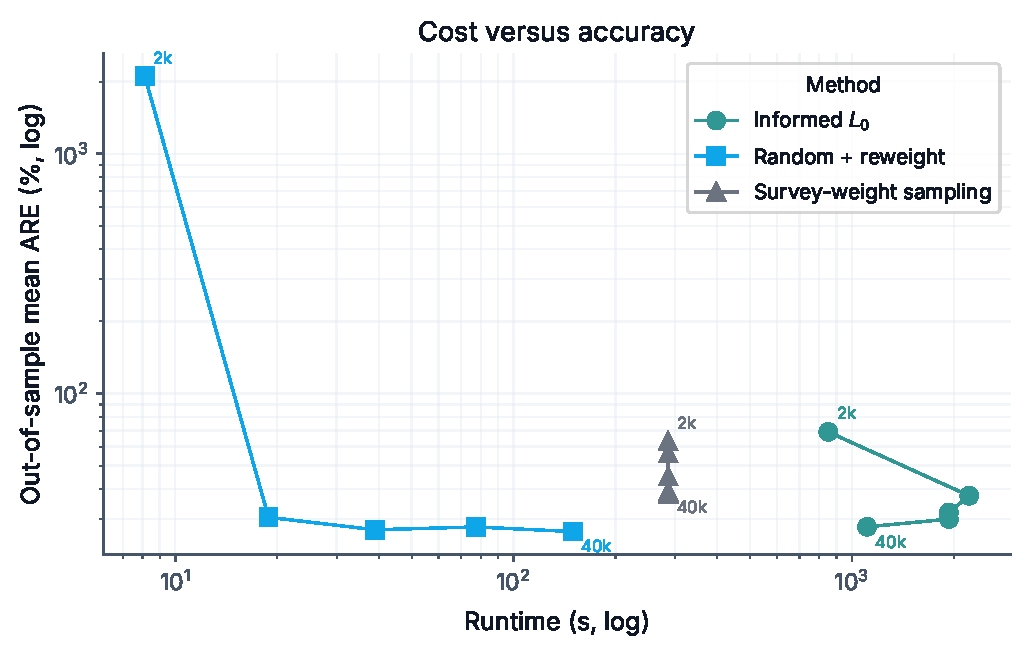
\includegraphics[width=0.8\textwidth]{figures/f5_cost_accuracy}
    \caption{Cost against accuracy: wall-clock runtime (log scale) against full-surface median ARE (log
    scale) for the four methods, each point labelled by its requested record budget. Informed $L_0$ and
    informed $L_0$ plus refit runtimes include the eight-step budget bisection that sets the sparsity
    penalty; the matched baselines run once at the budget. Points are the mean over three seeds.}
    \label{fig:cost_accuracy}
\end{figure}


\end{document}
